\documentclass[10pt]{beamer}
\usetheme[
%%% option passed to the outer theme
%    progressstyle=fixedCircCnt,   % fixedCircCnt, movingCircCnt (moving is deault)
  ]{Feather}

% If you want to change the colors of the various elements in the theme, edit and uncomment the following lines

% Change the bar colors:
%\setbeamercolor{Feather}{fg=red!20,bg=red}

% Change the color of the structural elements:
%\setbeamercolor{structure}{fg=red}

% Change the frame title text color:
%\setbeamercolor{frametitle}{fg=blue}

% Change the normal text color background:
%\setbeamercolor{normal text}{fg=black,bg=gray!10}

%-------------------------------------------------------
% INCLUDE PACKAGES
%-------------------------------------------------------

\usepackage[utf8]{inputenc}
\usepackage[english]{babel}
\usepackage[T1]{fontenc}
\usepackage{helvet}
\usepackage{listings}

%-------------------------------------------------------
% DEFFINING AND REDEFINING COMMANDS
%-------------------------------------------------------

% colored hyperlinks
\newcommand{\chref}[2]{
  \href{#1}{{\usebeamercolor[bg]{Feather}#2}}
}

%-------------------------------------------------------
% Configure syntax highlight
%-------------------------------------------------------
\lstset{
  backgroundcolor=\color{white},
  breaklines=true,
  commentstyle=\color{green},
  extendedchars=true,
  frame=single,
  keepspaces=true,
  keywordstyle=\color{blue},
  language=Ruby,
  numbers=left,
  numbersep=10pt,
  numberstyle=\small\color{gray},
  rulecolor=\color{black},
  stringstyle=\color{blue},
  tabsize=2
}

%-------------------------------------------------------
% INFORMATION IN THE TITLE PAGE
%-------------------------------------------------------

\title[] % [] is optional - is placed on the bottom of the sidebar on every slide
{ % is placed on the title page
      \textbf{Apache httpd}
}

\subtitle[Managements]
{
}

\author[Rodrigo Siqueira]
{      Rodrigo Siqueira\\
      {\ttfamily siqueira@kuniri.org}
}

\institute[]
{
      Institute of Mathematics and Statistics\\
      University of Sao Paulo\\

  %there must be an empty line above this line - otherwise some unwanted space
  % is added between the university and the country (I do not know why;( )
}

\date{\today}

%-------------------------------------------------------
% THE BODY OF THE PRESENTATION
%-------------------------------------------------------

\begin{document}

%-------------------------------------------------------
% THE TITLEPAGE
%-------------------------------------------------------

{\1% % this is the name of the PDF file for the background
% the plain option removes the header from the title page, noframenumbering removes the numbering of this frame only
\begin{frame}[plain,noframenumbering]
  \titlepage % call the title page information from above
\end{frame}}

\begin{frame}[shrink]{Content}{}
  \tableofcontents
\end{frame}

%=======================================================
\section{Introduction}
%=======================================================
\begin{frame}{Introduction}{What is Apache HTTPD?}
  \begin{figure}[ht]
    \centering
    
\includegraphics[width=1\textwidth, keepaspectratio=true]{images/apachehttpd.jpg}
  \end{figure}
\end{frame}

\begin{frame}{Introduction}{A brief history of httpd}
\end{frame}

%=======================================================
\section{How httpd project is organized}
%=======================================================
\begin{frame}{Introduction}{What is Apache HTTPD?}
  \begin{figure}[ht]
    \centering
    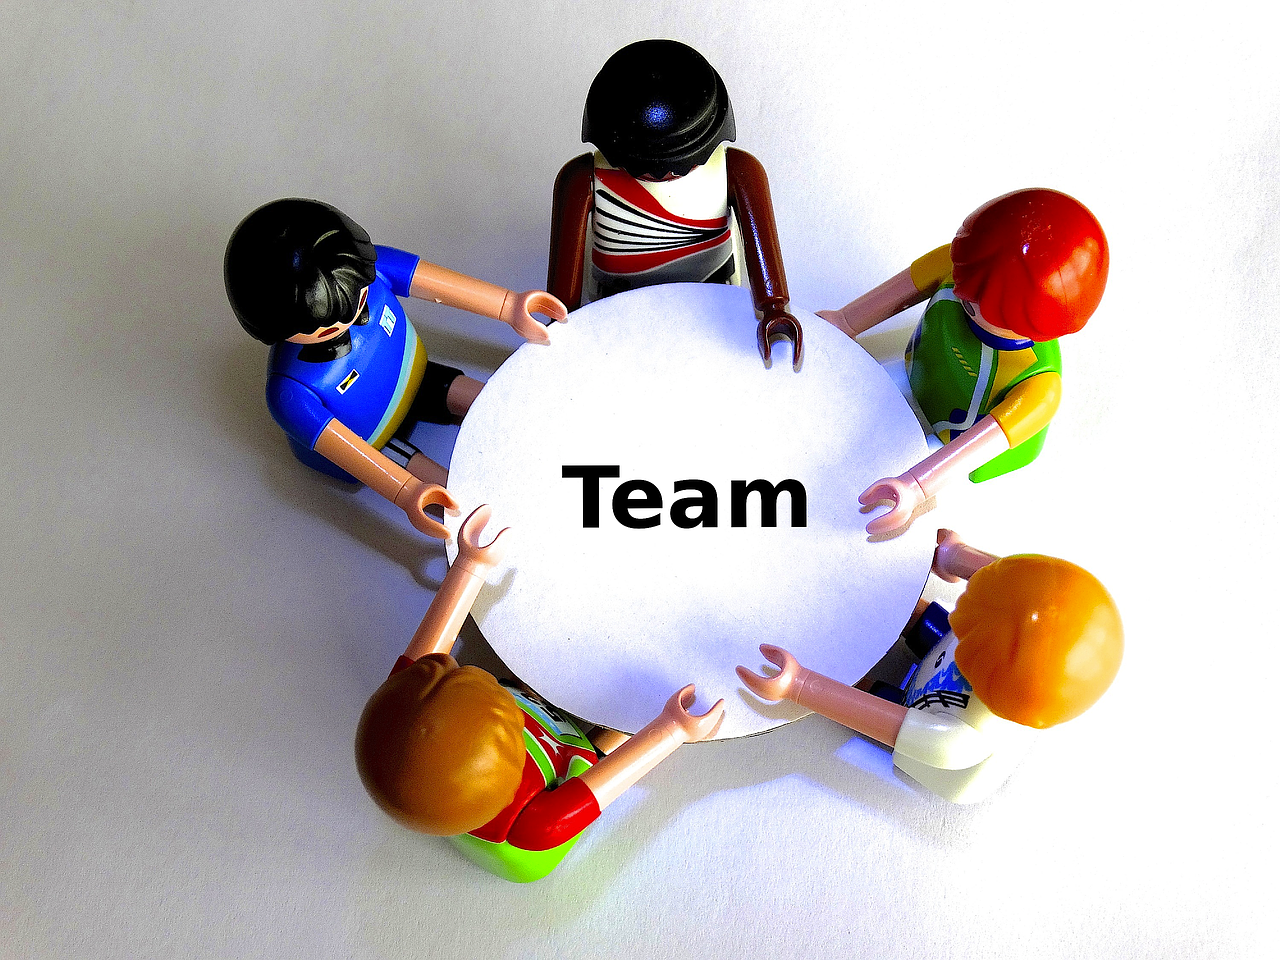
\includegraphics[width=0.9\textwidth, keepaspectratio=true]{images/roles.jpg}
  \end{figure}
\end{frame}

%-------------------------------------------------------
\subsection{Roles}
%-------------------------------------------------------
\begin{frame}{People, roles, etc}{Project Management Committee (PMC)}
  What it is Project Management Committee? \pause
  \begin{itemize}
    \item The group of volunteers who are responsible for managing the Apache
          HTTP Server Project \pause
  \end{itemize}

  What is their responsibilities? \pause
  \begin{itemize}
    \item What is distributed as products of the HTTPD \pause
    \item Maintaining the project's shared resources \pause
    \item Maintaining the project's resources \pause
    \item Speaking on behalf of the project \pause
    \item Resolving license disputes \pause
    \item Nominating the new PMC members or committers \pause
    \item Establishing guidelines
  \end{itemize}
\end{frame}

\begin{frame}{People, roles, etc}{Committers}
  \begin{figure}[ht]
    \centering
    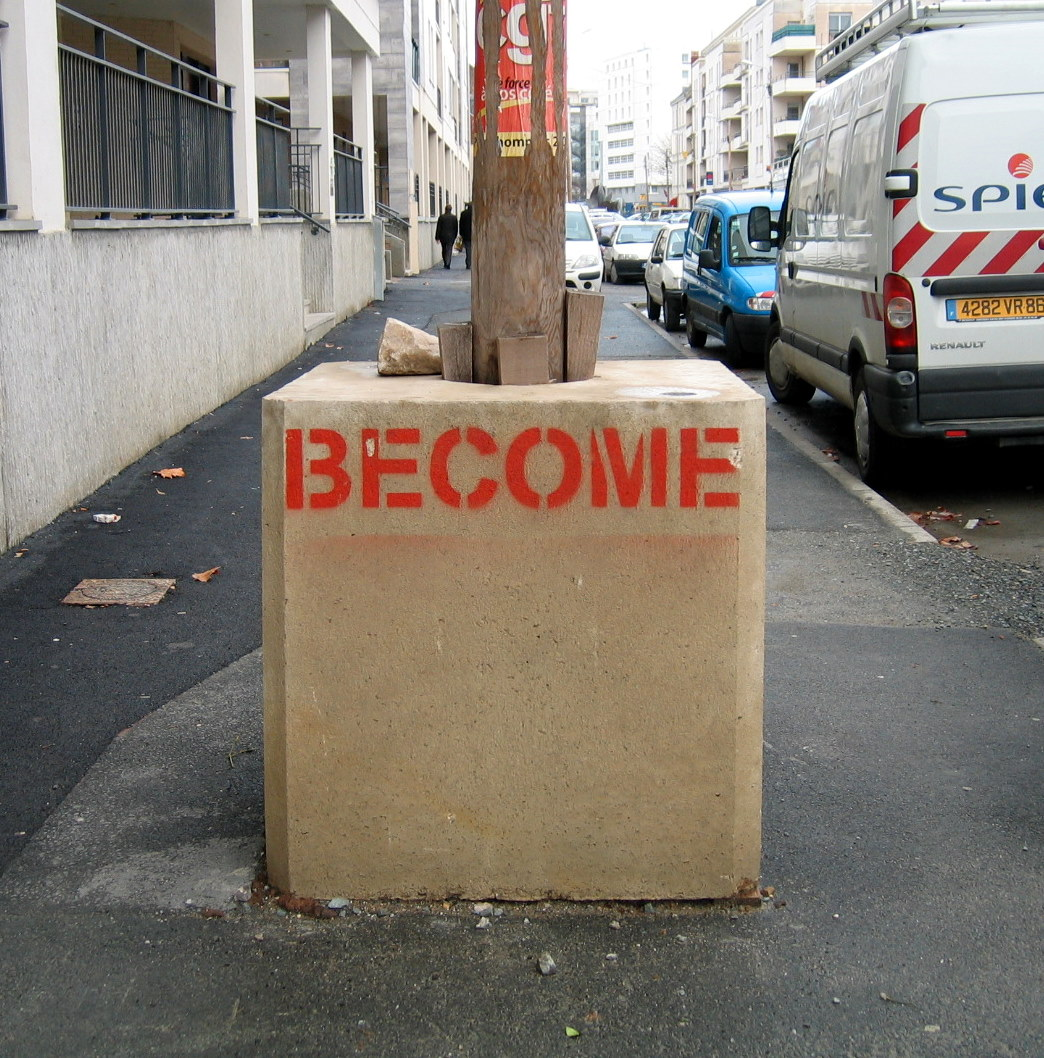
\includegraphics[width=0.6\textwidth, keepaspectratio=true]{images/become.jpg}
  \end{figure}
\end{frame}

\begin{frame}{People, roles, etc}{Committers}
  How to become an Apache committer? \pause
  \begin{itemize}
    \item First of all, you need to use Apache as a user \pause
    \item Enjoy to the mailing list \pause
    \item Submit your patches and wait for review \pause
    \item Meritocracies:
    \begin{itemize}
      \item If you contribute to the project frequently, a membership can
            invite you \pause
      \item After you receive the invitation, PMC will vote to approve or not
            to give you permission \pause
      \item Usually, if you contribute frequently for six month you can receive
            an invitation
    \end{itemize}
  \end{itemize}
\end{frame}

\begin{frame}{People, roles, etc}{Release Manager}
  \begin{figure}[ht]
    \centering
    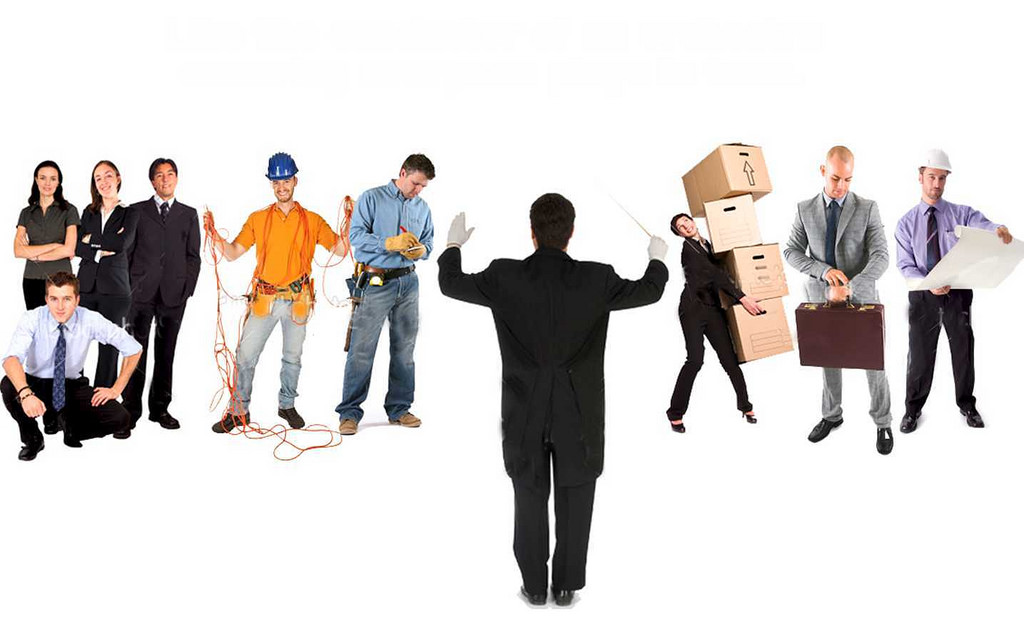
\includegraphics[width=0.7\textwidth, keepaspectratio=true]{images/release_management.jpg}
  \end{figure}
\end{frame}

\begin{frame}{People, roles, etc}{Release Manager}
  What is a Release Manager (RM)? \pause
  \begin{itemize}
    \item Someone (or group) responsible for release new versions \pause
  \end{itemize}

  What is their responsibilities? \pause
  \begin{itemize}
    \item Coordinate development community \pause
    \item Alert the community about the planned release schedule
  \end{itemize}
\end{frame}

%=======================================================
\section{Releases}
%=======================================================
\begin{frame}{Releases}{How it works?}
  \begin{figure}[ht]
    \centering
    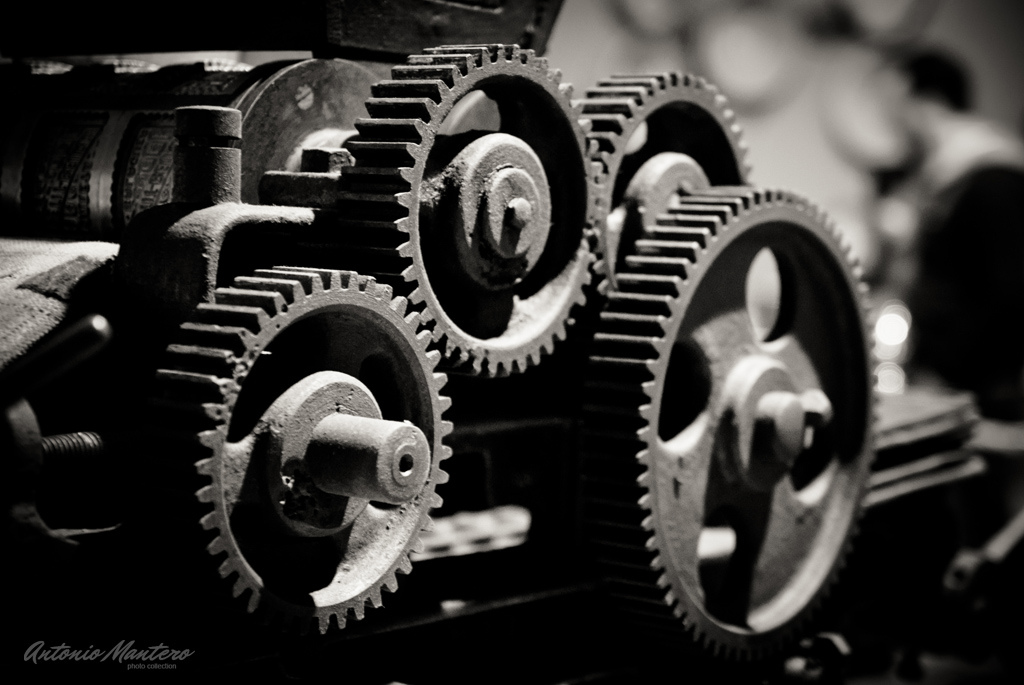
\includegraphics[width=0.9\textwidth, keepaspectratio=true]{images/gears.jpg}
  \end{figure}
\end{frame}

\begin{frame}{Releases}{How it works?}
  \begin{itemize}
    \item Odd-even release strategy. Example: \pause
    \begin{itemize}
      \item Development happens with alpha and beta releases assigned an
            odd-numbered minor version. \pause
      \item General availability (stable) release is designed with the
            subsequent event-numbered minor version \pause
      \item 2.1.0-alpha, 2.1.6-alpha, 2.1.7-beta, 2.2.0 \pause
    \end{itemize}

    \item How can make a release? \pause
      \begin{itemize}
        \item Anyone can make a release of the source code \pause
        \item However, only members of the Apache HTTPD can make a release
              designated as Apache httpd
      \end{itemize}
  \end{itemize}
\end{frame}

\begin{frame}{Releases}{How is in charge of a release?}
  \begin{figure}[ht]
    \centering
    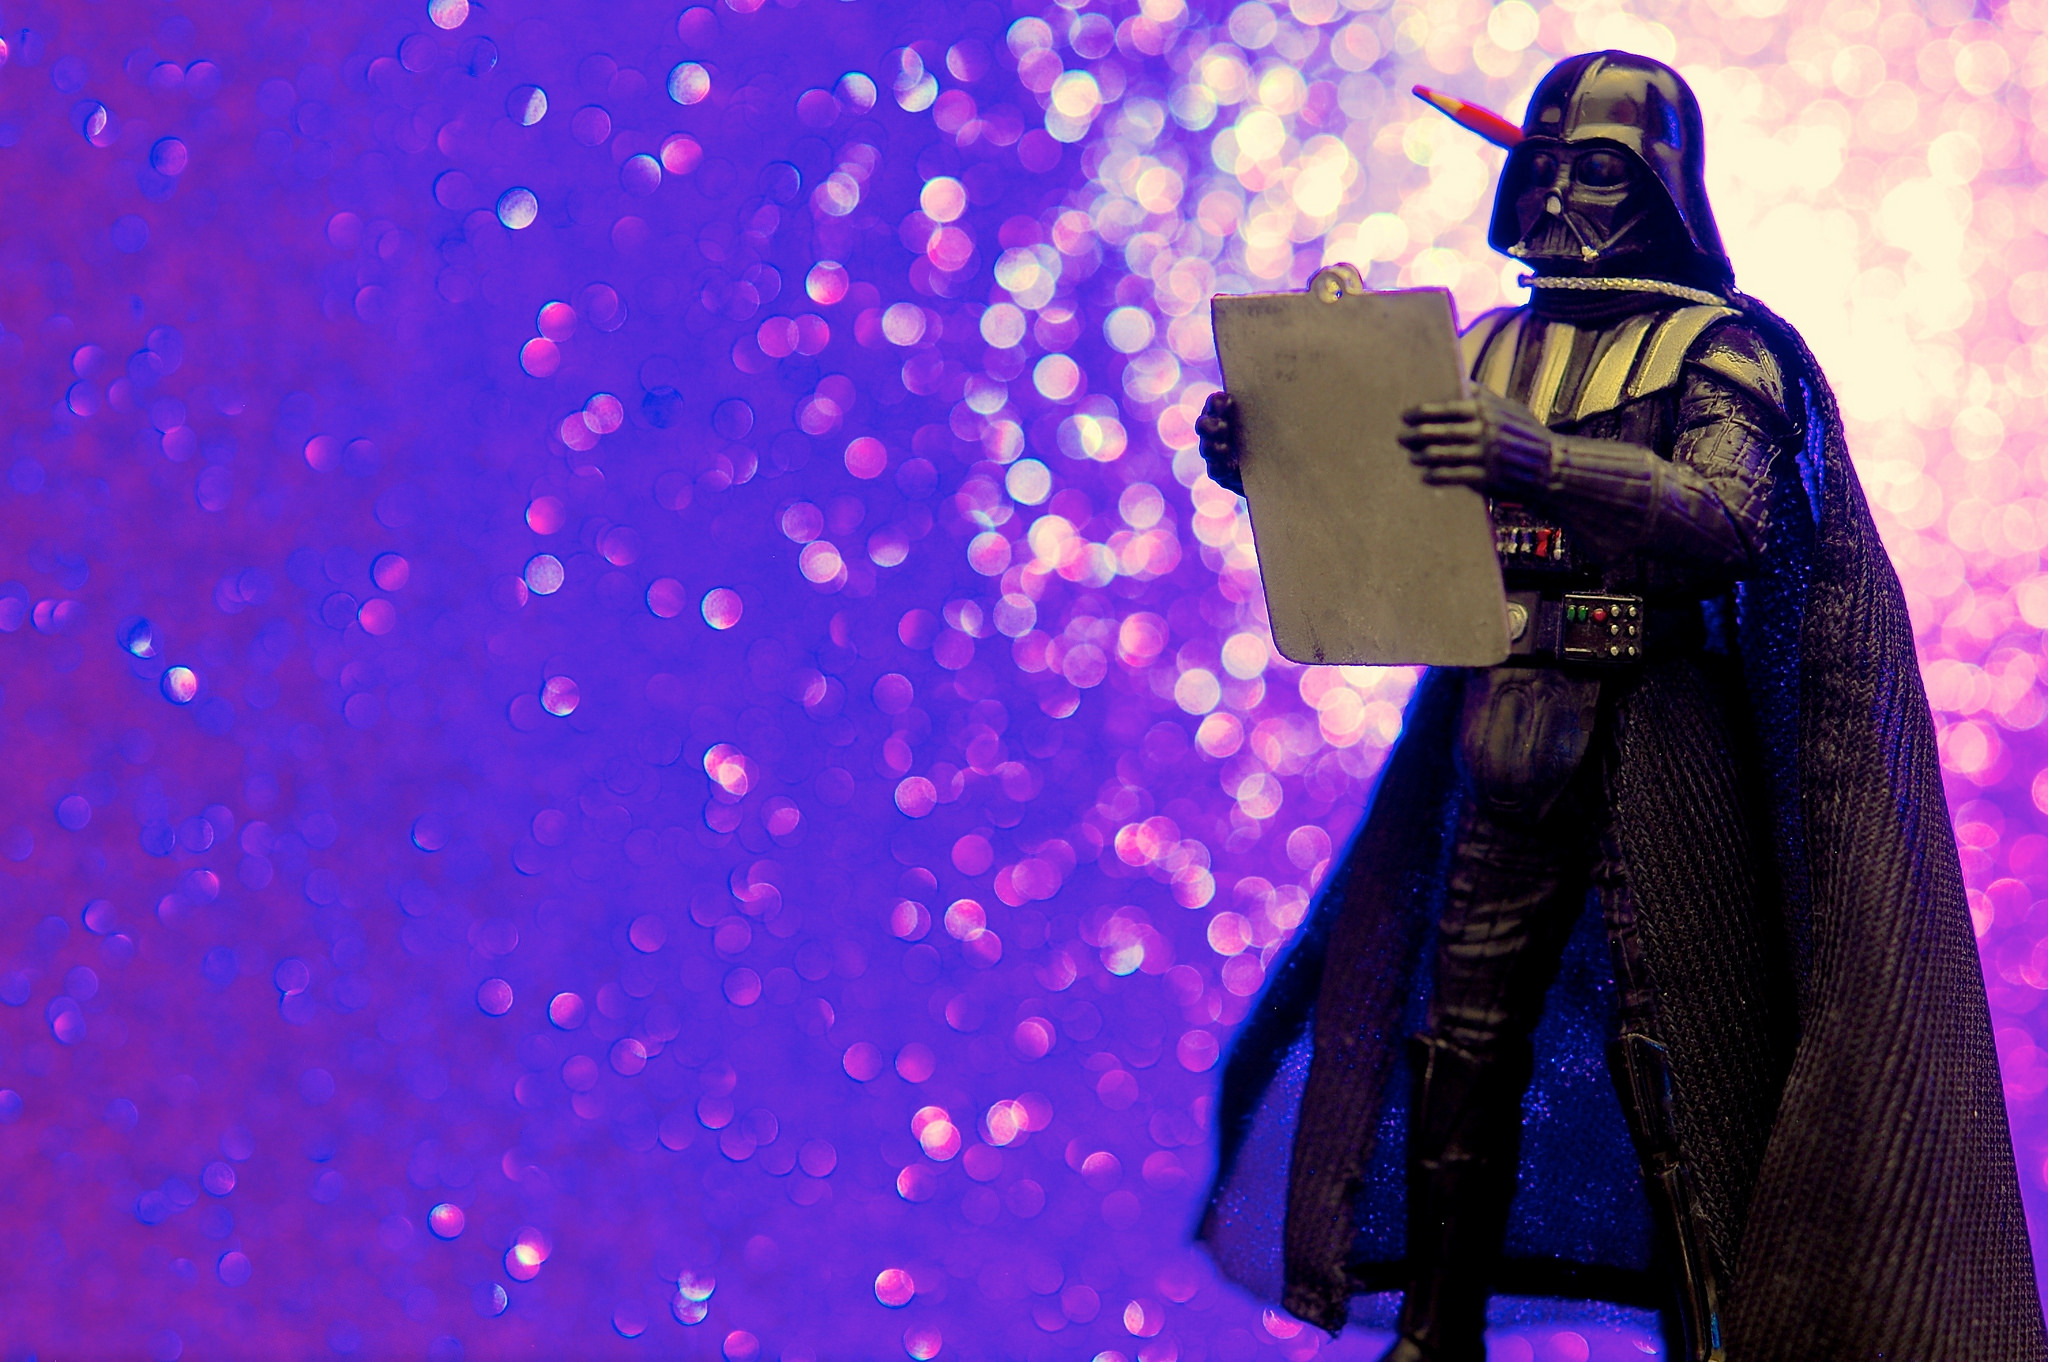
\includegraphics[width=0.8\textwidth, keepaspectratio=true]{images/rm.jpg}
  \end{figure}
\end{frame}

\begin{frame}{Releases}{How is in charge of a release?}
  \begin{itemize}
    \item Basically, the Release Manager (RM) \pause
    \item This job requires trust, coordination of the development community,
          and access to subversion \pause
    \item Only committers to the project can be RM \pause
    \item More than one RM can be active at a time \pause
    \item A good candidate should have lots of time to kill \pause
    \item The only thing the RM has authority over is the building of a
          source package, based on the contents of subversion \pause
    \item The RM is not a dictator (benevolent or not)
  \end{itemize}
\end{frame}

%=======================================================
\section{Plain}
%=======================================================

%-------------------------------------------------------
\subsection{Status and Voting}
%-------------------------------------------------------

\begin{frame}{Plain}{Status}
  \begin{figure}[ht]
    \centering
    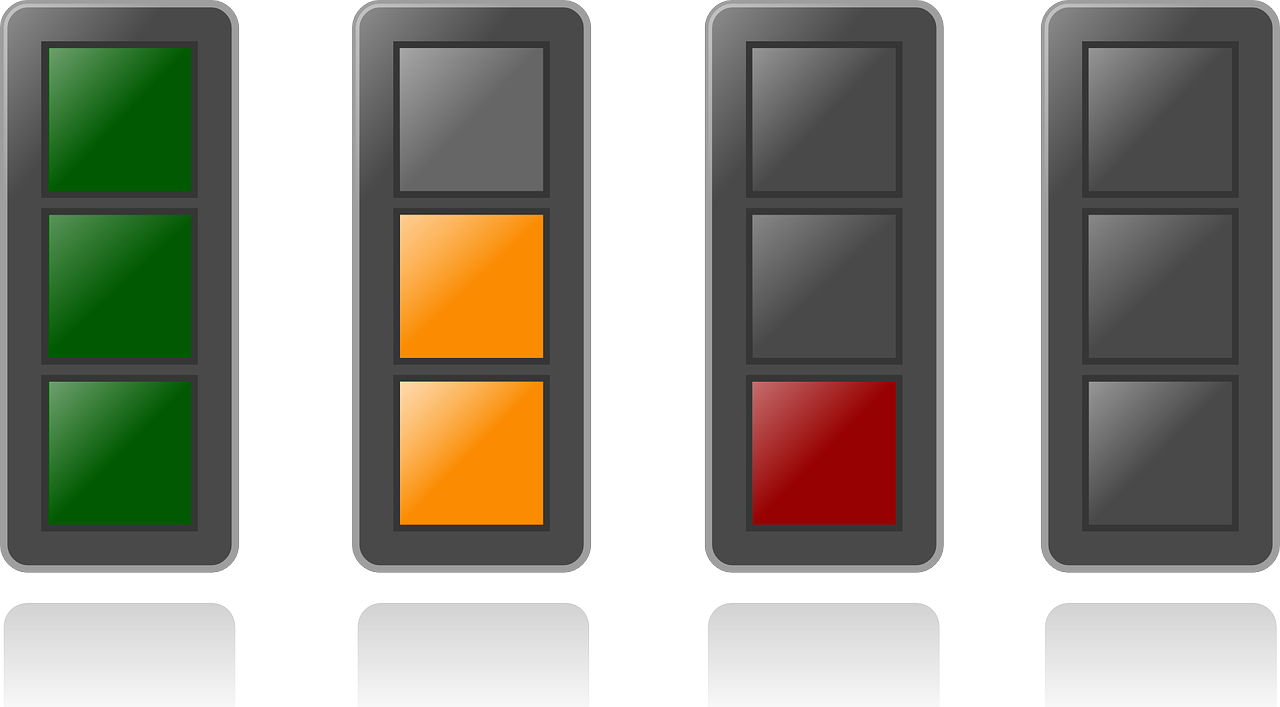
\includegraphics[width=0.5\textwidth, keepaspectratio=true]{images/status.png}
  \end{figure}
\end{frame}

\begin{frame}{Plain}{Status}
  What is Status file? \pause
  \begin{itemize}
    \item This file contains the track of the agenda and plans for work within
          that repository \pause
    \item Information about release plans \pause
    \item A summary of code changes committed since the last release
  \end{itemize}
\end{frame}

\begin{frame}{Plain}{Voting}
  \begin{figure}[ht]
    \centering
    
\includegraphics[width=0.4\textwidth, keepaspectratio=true]{images/vote.jpg}
  \end{figure}
\end{frame}

\begin{frame}{Plain}{Voting}
  How decisions are taken in Apache? \pause
  \begin{itemize}
    \item Voting on any issue or action item
  \end{itemize}

  How voting works in Apache? \pause
  \begin{itemize}
    \item Any of the Apache Developers may vote on any issue or action
          item \pause
    \item Only binding votes are those cast by active members of the
          Apache \pause
    \item If the vote is about a change to source code or documentation,
          the primary author of what is being changed may also cast a binding
          vote \pause
    \item An action item requiring consensus approval must receive at least 3
          binding +1 votes and no vetos \pause
    \item Lazy approval
  \end{itemize}
\end{frame}

%-------------------------------------------------------
\subsection{Types of Action items}
%-------------------------------------------------------
\begin{frame}{Pain}{Types of Action items}
  \begin{itemize}
    \item Long term Plans
    \item Short therm Plans
    \item Release Plan
    \item Release Testing
    \item Showstoppers
    \item Product Changes
    \item An idea or plan for a change
    \item Proposed patch
    \item Committed change
  \end{itemize}
\end{frame}

\begin{frame}{Plain}{Voting}
  \begin{figure}[ht]
    \centering
    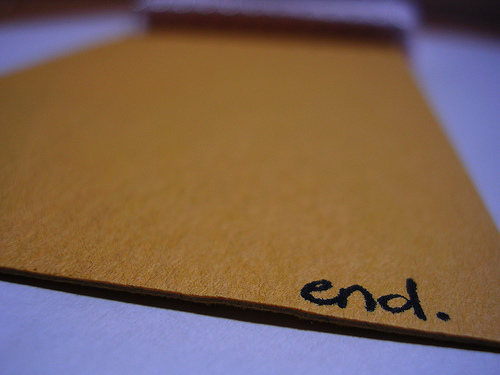
\includegraphics[width=0.6\textwidth, keepaspectratio=true]{images/end.jpg}
  \end{figure}
\end{frame}


%=======================================================
\section{References}
%=======================================================

\begin{frame}{References}{References}
  \begin{itemize}
    \item Apache guideline
    \item Apache Release guideline
  \end{itemize}
\end{frame}

\end{document}
